% Slide 13 -- Qualitative results: full-figure
\begin{frame}{Qualitative results: per-dataset summary}
  \centering
  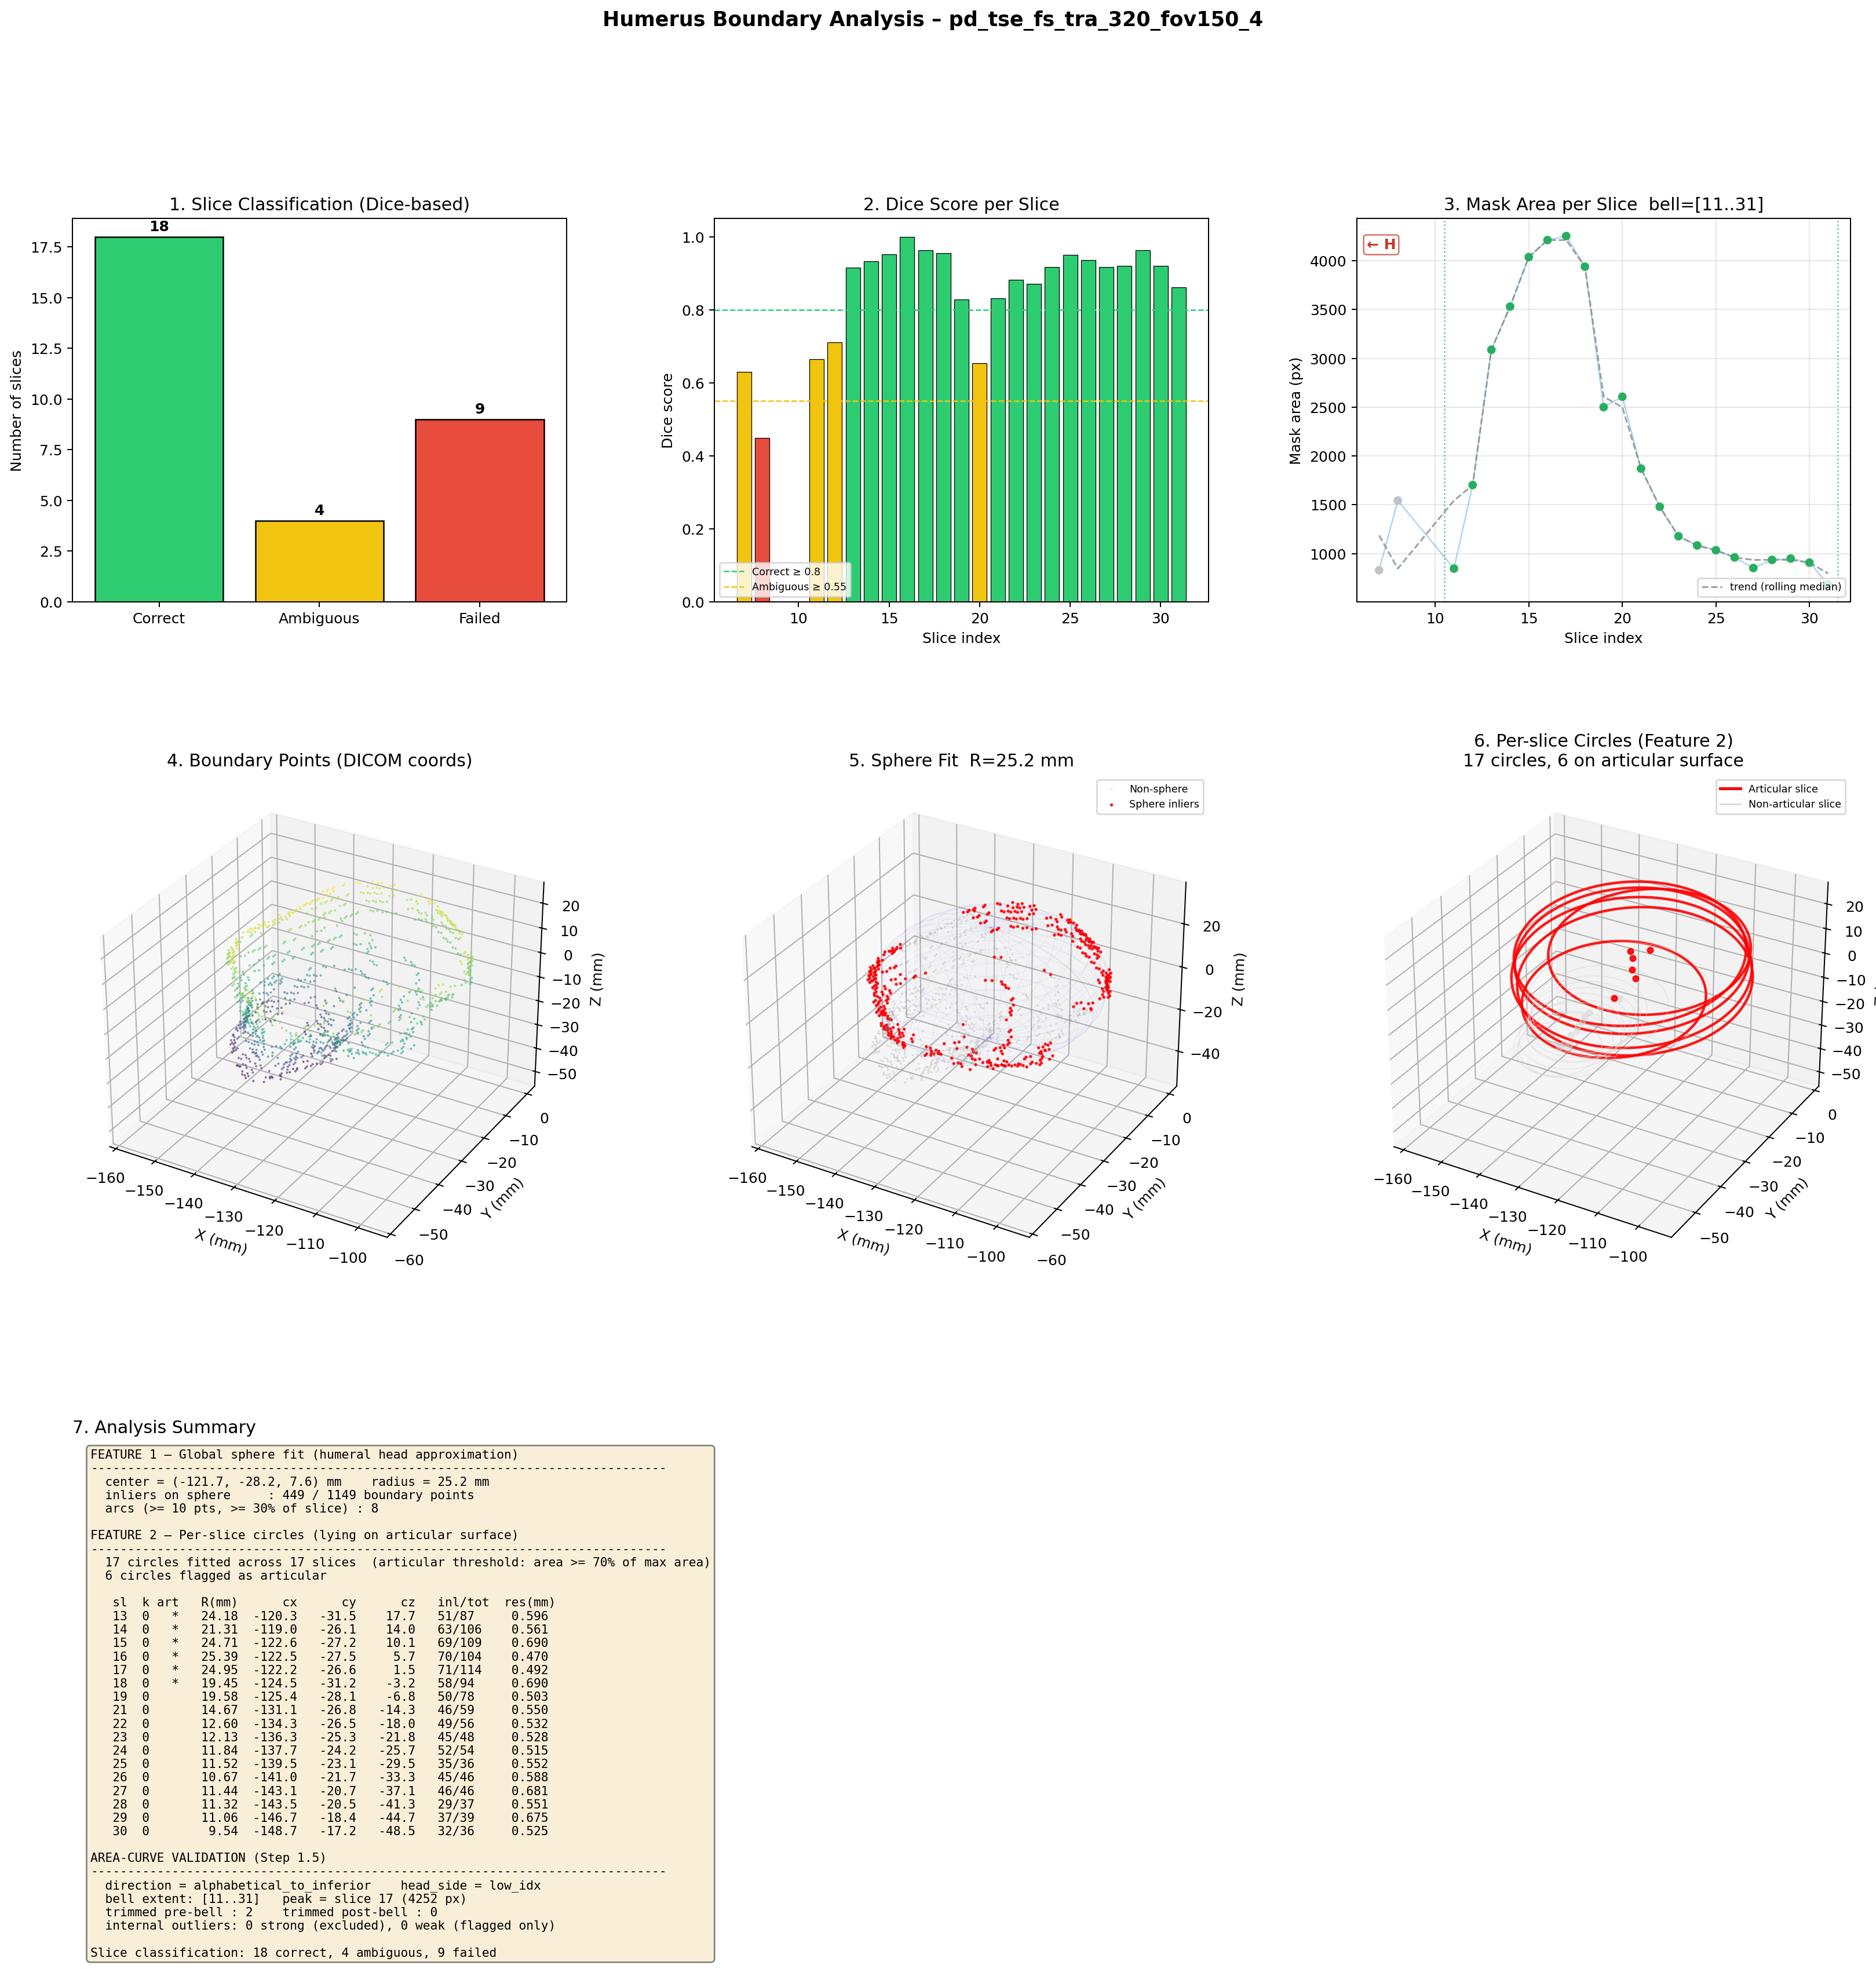
\includegraphics[height=0.75\textheight,keepaspectratio]{figures/summary_pd4.png}
  \\[0.3em]
  {\footnotesize Summary for dataset \textit{pd\_tse\_fs\_tra\_320\_fov150\_4}: mask boundaries,
  area curve with Step 1.5 status, slice-circle centers and reconstructed surface.}
\end{frame}

% Slide 13b -- How to read the figure
\begin{frame}{How to read the summary figure}
  \begin{columns}[T]
    \begin{column}{0.55\textwidth}
      \begin{block}{Color code (panel 3, area curve)}
        \begin{itemize}
          \item \textcolor{green!50!black}{\textbf{Green}}: slices kept for analysis.
          \item \textcolor{gray}{\textbf{Gray}}: tails trimmed by direction-aware logic.
          \item \textcolor{red}{\textbf{Red}}: strong outliers excluded after Pass 2.
          \item Vertical lines: bell-extent boundaries.
          \item Caret \texttt{H$\rightarrow$}: which side of the volume is the head.
        \end{itemize}
      \end{block}
    \end{column}
    \begin{column}{0.45\textwidth}
      \begin{block}{Auditability by design}
        Every slice exports a five-panel \texttt{*\_circle.png} (image, mask, contour, fitted circle, overlay). A radiologist can verify each fit \alert{slice by slice}, not just trust an aggregate score.
      \end{block}

      \begin{block}{Reproducibility}
        All thresholds are exposed as CLI flags;
        every run writes \texttt{area\_curve\_validation.csv} for downstream audit.
      \end{block}
    \end{column}
  \end{columns}
\end{frame}
